\begin{figure}[htbp]
\centering
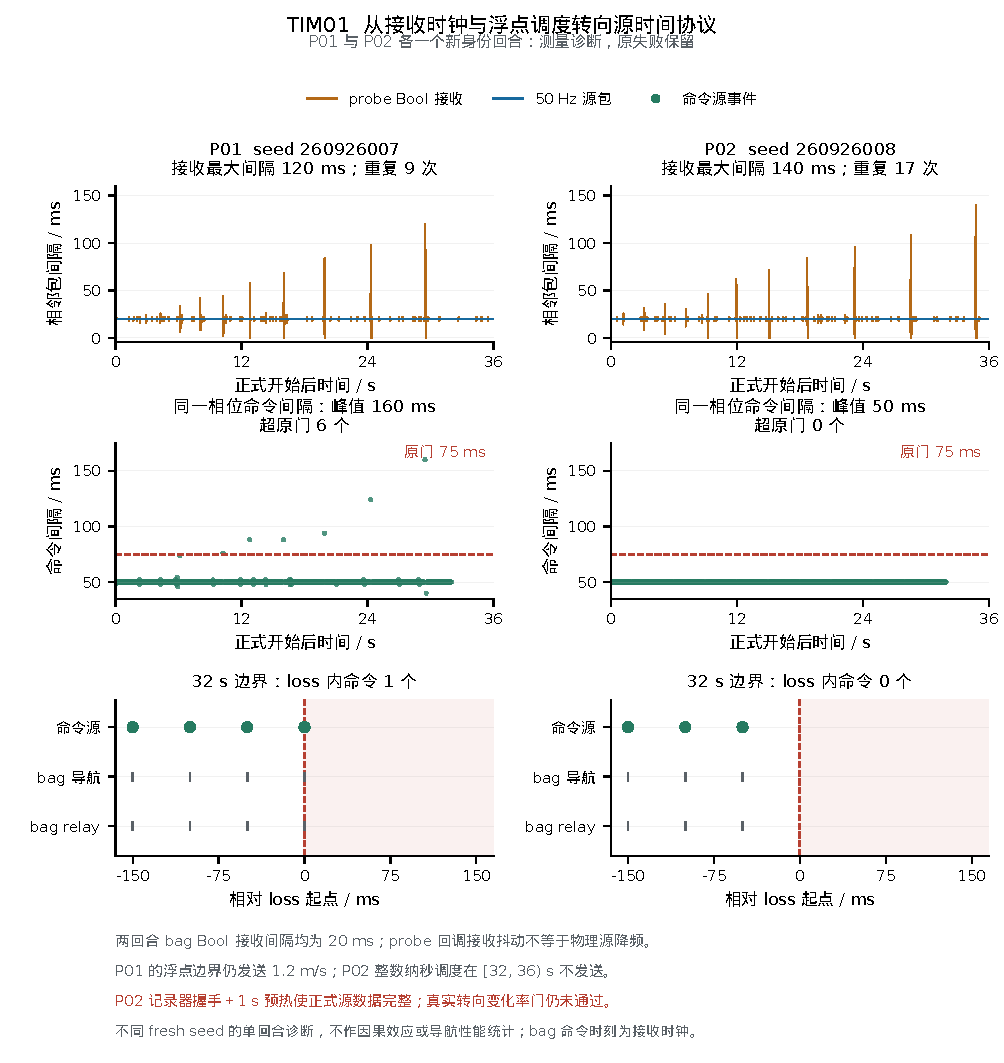
\includegraphics[width=170mm]{TIM01.pdf}
\caption{P01与P02测量通道和命令时序的离线诊断。两列来自各自独立的新seed单回合，不能用于估计修复的统计因果效应。上排比较probe无Header Bool回调接收时钟与具有Header的50Hz源包；P01源包用actuator_target，P02用physical_status。接收最大间隔分别为120/140ms、重复接收时刻9/17次，但两次bag Bool接收最大间隔均为20ms，说明回调调度抖动不能直接解释为物理发布降频。中排展示同一相位内全部相邻命令间隔，P01/P02峰值160/50ms，超过冻结75ms门6/0个；故意无命令的loss段不作为“丢帧”计算。下排显示32s整数loss起点附近的全部源命令事件及bag导航/relay接收，P01仍在边界发送1.2m/s，P02在[32,36)s严格不发送。P01原Bool完整性失败保持，其AST诊断另外保留命令间隔、loss边界及实际转向变化率失败；P02正式源流和命令协议通过，但实际20ms中心角变化率0.88636rad/s仍超过0.85rad/s门。P01起始bag缺包与P02完整覆盖的独立审计见引用数据SHA。源事件时刻为Python publish前采样；bag导航、relay和Bool时刻为接收时钟，不视为真实驱动接收时间。}
\label{fig:tim01-measurement-clock}
\end{figure}
